\documentclass[a4paper,12pt,twocolumn]{extarticle}
\usepackage[utf8]{inputenc}
\usepackage[paper=a4paper,left=24mm,right=24mm,top=20mm,bottom=20mm]{geometry}
\usepackage[svgnames]{xcolor}
\usepackage[spanish]{babel}
\usepackage{titlesec}
\usepackage{amsmath}
\usepackage{amsfonts}
\usepackage{csquotes}
\usepackage{enumitem}
\usepackage{tcolorbox}
\usepackage{titling}
\usepackage{hyperref}
\usepackage[sorting=none]{biblatex}
\usepackage{tgheros} 
\usepackage{tikz}
\usepackage{pgfplots}
\usepackage{minted}

\setminted[python]{
    % fontsize=\footnotesize,
    fontsize=\scriptsize,
    breaklines
}

\hypersetup{
    colorlinks=true
}

% enumitem config
\renewcommand\labelitemi{--}
\setlist[itemize]{itemsep=0em}

% Redefining titles
\titleformat{\section}{\mdseries\Large\sffamily}{\thesection. }{0em}{\Large\mdseries\sffamily}
\titleformat{\subsection}{\large\sffamily}{\thesubsection. }{0em}{\large\sffamily}
\titleformat{\subsubsection}{\sffamily}{\thesubsubsection. }{0em}{\sffamily}

% New commands 
\newcommand*{\email}[1]{\normalsize\href{mailto:#1}{#1}}
\newcommand{\projectloc}{\href{https://github.com/Irulam/Trading-cuantitativo-cuantico}{ GitHub }}
\makeatletter
\newcommand{\forceonecolumn}[1]{
    \if@twocolumn\twocolumn[
        \begin{@twocolumnfalse}
        #1
        \end{@twocolumnfalse}
    ]
    \else
        #1
    \fi
}
\makeatother
\newtcolorbox{resultado}[1][]{
    boxrule=0pt, arc=0pt,
    left=3pt, right=3pt, boxsep=0pt,
    colframe=black, colback=Gainsboro,
    fontupper=\scriptsize,
    #1,
}

%%%% COSAS DE TIKZ
\usetikzlibrary{arrows}
\usetikzlibrary{calc}
\usetikzlibrary{positioning}
\tikzset{>=stealth}
\pgfmathdeclarefunction{gauss}{2}{\pgfmathparse{1/(#2*sqrt(2*pi))*exp(-((x-#1)^2)/(2*#2^2))}}
\pgfmathdeclarefunction{lognormal}{2}{\pgfmathparse{1/(x*#2*sqrt(2*pi))*exp(-((ln(x)-#1)^2)/(2*#2^2))}}

% \title{\sffamily\bfseries Apliaciones Financieras\\ de la Computación Cuántica}
\title{\sffamily\bfseries Valoración de Instrumentos Financieros Derivados mediante Computación Cuántica}
\date{\today{}}
\author{David Davó Laviña\\\email{ddavo@ucm.es}\and Leidy Vanesa Vidales González\\\email{leidyvid@ucm.es}}

\addbibresource{bibliografia.bib}

\begin{document}
\forceonecolumn{
    \maketitle
    \begin{abstract}
    Un concepto interesante en la computación cuántica es el ``aventajamiento cuántico" \cite{Egger2020}, consistente en buscar aplicaciones en las que la ejecución de algoritmos cuánticos consiga un \textit{speedup} considerable con respecto a su equivalente clásico. En la actualidad, contamos con varias herramientas de programación cuántica, pero usadas principalmente en investigación. Sin embargo, su integración en los flujos de trabajo de las empresas es inminente, hacia principios de 2023 según IBM \cite{wehden_faro_gambetta_2021}.
    
    Este aventajamiento puede notarse pronto por ejemplo en la simulación, en la que pasaríamos de hacer simulaciones clásicas de Monte Carlo a usar estimaciones de amplitud, con una mejora cuadrática.
    \end{abstract}
}

\section{Introducción}

Siguiendo esta memoria y el Jupyter Notebook adjunto aprenderemos a valorar opciones financieras, pasando por una explicación de sus fundamentos y su valoración en computadores clásicos. Finalmente, resolveremos el cálculo del valor estimado de una opción usando Qiskit \cite{Qiskit} Aqua. Podéis encontrar el Jupyter Notebook y el código fuente de este documento en el \projectloc del proyecto.

\section{Introducción a las finanzas}
\label{sec:introfinance}

Esta sección esta basada principalmente en \cite{wilmott_howison_dewynne_1995} y \cite{10.5555/1370958}

Podemos distinguir distintos tipos de mercados financieros:
\begin{itemize}
    \item \textbf{Mercado de valores} o \textit{stock market}: Se intercambian acciones o \textit{stocks} de empresas
    \item \textbf{Bonos}: Se comercia con deuda de gobiernos o empresas
    \item \textbf{Forex}: Mercados basados en el intercambio de la moneda de distintos países
    \item \textbf{Comodidades:} Se comercia con activos físicos como el petróleo, el oro o el trigo
    \item \textbf{Mercado a término:} Se comercia con productos financieros derivados, que se basan en el precio de otro activo como \textbf{futuros} y \textbf{opciones}.
\end{itemize}

Varios de estos mercados pueden ser accesibles mediante una organización pública o privada llamada Bolsa de Valores que estandariza y facilita el comercio de Instrumentos Financieros entre compradores y vendedores.

A continuación explicaremos con más detalle el mercado de valores y los futuros y opciones, que luego optimizaremos en Qiskit.

\subsection{Mercado de valores}
Se comercia con uno de los instrumentos financieros más básicos, llamados equidad, \textit{stock}, participación o valor. Un inversor da capital a una compañía, y a cambio pasas a ser propietario de una parte de la compañía. El conjunto de personas que invierten en una compañía se denomina \textit{shareholders} o accionistas, y técnicamente tienen cierto poder de decisión en las operaciones que realice la empresa. Los directores de la compañía deben servir a los intereses de los accionistas. Cada accionista también recibirá \textit{dividendos} en un periodo de tiempo determinado, por ejemplo cada trimestre, cada año, o cada 6 meses. Además, en cualquier momento puedes decidir vender tu acción (ya sea en una bolsa de valores, o de forma externa, conocido como OTC o \textit{Over The Counter}), por lo que puedes ganar dinero si inviertes en una empresa con acciones a un precio bajo, y vendes las acciones cuando su valor sube.

\subsection{Futuros y forwards}
Los \textbf{futuros} y los \textbf{forwards} son Instrumentos Financieros Derivados, es decir, su valor depende del valor de otro instrumento financiero. En este caso, de una acción. Ambos son contratos en los que una parte promete comprar a un activo a otra parte en un tiempo determinado (fecha de entrega o madurez) a un precio acordado llamado precio de entrega. 

Los contratos \textbf{forward} son acuerdos privados (OTC o \textit{Over The Counter}) en los que
el precio del activo está determinado en el momento del contrato. Cuando llega la fecha de entrega, debemos comprar la acción al precio de entrega, sea este mayor o menor que el precio actual de mercado de la acción.

Un contrato de \textbf{futuro} es muy similar al contrato forward, pero están regulados por mercados de futuros (es decir, en una bolsa de valores) y además su valor se va ajustando diariamente, por lo que el precio de entrega en la fecha de entrega es igual al precio de mercado.

Tanto futuros como forwards pueden usarse para \textit{especulación}, en la que ``apuestas"  sobre la dirección en la que se moverá el precio de un activo. Puedes \textit{ir largo} y, cuando recibas el activo llegado el tiempo de entrega, puedes venderlo inmediatamente para recibir un beneficio. También tienes la opción de \textit{ir corto} y vender el activo (que aún no posees) mientras que estableces un contrato de futuro.
Otra posible operación es el \textit{hedging} o cobertura, que consiste en disminuir el riesgo invirtiendo en un activo financiero relacionado con el que ya se ha invertido de tal forma que respalde a una posible pérdida. 

\subsection{Opciones}
Son derivados financieros. Podemos distinguir dos tipos de opciones, las opciones de venta (\textit{calls}) y las opciones de compra (\textit{puts}). Mientras que el titular de un contrato de futuro está \textbf{obligado} a liquidar el activo subyacente llegada la madurez del contrato (a no ser que se cierre antes de la fecha de entrega), en las opciones obtenemos el \textit{derecho} a comprar/vender a un precio determinado llamado \textit{precio de ejercicio} o \textit{strike} antes de una fecha determinada llamada \textit{fecha de vencimiento}.

Por ejemplo, si compramos una opción con fecha de vencimiento dentro de un año por 100€, y el día de la fecha de vencimiento el precio de mercado del activo subyacente es de 120€, podemos ejecutar la opción, comprar el activo y venderlo inmediatamente, obteniendo un beneficio de 20€.

Siendo $V$ el valor de la acción en la fecha de vencimiento, y sea $E$ el precio de ejercicio, podemos definir nuestro beneficio al vencimiento con la siguiente función, llamada pago (\textit{payoff}):
\begin{equation}
    \label{eq:optionput}  
    \max\left(V-E, 0\right)
\end{equation}

Es decir, cuando el precio de ejercicio (\textit{spot price}) es mayor que el precio de vencimiento (\textit{strike price}), decidimos no ejecutar la opción, porque no obtendríamos ningún beneficio.

Análogamente en una opción de venta tendríamos la siguiente:
\begin{equation}
    \label{eq:optioncall}
    \max\left(E-V, 0\right)
\end{equation}

Estas funciones se denominan funciones de recompensa y nos indican el beneficio que podemos obtener con un activo dependiendo de determinados parámetros.

Podemos distinguir dos tipos de opciones:
\begin{itemize}
    \item \textbf{Europeas}: El ejercicio sólo se permite en la fecha de vencimiento
    \item \textbf{Americanas}: El ejercicio se permite en cualquier momento antes de la fecha de vencimiento
\end{itemize}

Nos vamos a fijar principalmente en las opciones Europeas al ser más sencillas. Nuestro objetivo será valorar el valor de la opción antes de comprarla, y para ello intentaremos predecir dentro de un intervalo de confianza el valor del subyacente en el tiempo de expiración.

\subsubsection{Modelo Binomial}
Existen muchos métodos para intentar calcular el valor de un activo en un tiempo determinado, siendo el más simple el modelo binomial o BOPM (\textit{Binomial Options Pricing Model}).

En el modelo binomial suponemos que el activo puede subir o bajar de valor en unas cantidades determinadas $u$ y $d$ de un día al siguiente, con una probabilidad $p$. Sin entrar a cómo calcular estos parámetros, generamos un árbol de probabilidades de la misma manera que hacíamos en el instituto, iterativamente, hasta llegar a la fecha de vencimiento. Tendremos por lo tanto un árbol con las distintas trayectorias: ``Todos los días sube'', ``El primer día sube, el siguiente baja, luego sube...'', ``Todos los días baja'', ``Sube dos de cada tres días'', etc. Nuestro árbol tendrá por lo tanto $2^n$ ramas, siendo n el número de días que hayan pasado, o la profundidad del árbol. 

\begin{figure}[h]
    \centering
    % \resizebox{\textwidth}{!}{\include{}
    \begin{tikzpicture}[
        node distance=4mm and 14mm,
        label distance=-2mm,
        every node/.style={circle,fill=black,inner sep=0pt,minimum size=5pt},
        every path/.style={very thick,-stealth}
    ]
    \node[label=above:{30.00€}] (r) {};
    
    \node[above right=of r,label=above:{\footnotesize 31.50€}] (u) {};
    \node[below right=of r,label=above:{\footnotesize 28.57€}] (d) {};
    
    \path[green] (r) edge (u);
    \path[red]   (r) edge (d);
    
    \node[above right=of u,label=above:{\footnotesize 33.08€}] (uu) {};
    \node[above right=of d,label=above:{\footnotesize 30.00€}] (du) {};
    \pgfnodealias{ud}{du}
    \node[below right=of d,label=above:{\footnotesize 27.21€}] (dd) {};

    \path[green] (u) edge (uu);
    \path[green] (d) edge (du);
    \path[red]   (u) edge (ud);
    \path[red]   (d) edge (dd);
    
    \node[above right=of uu,label=above:{\footnotesize 34.73€}] (uuu) {};
    \node[above right=of du,label=above:{\footnotesize 31.50€}] (duu) {};
    \node[above right=of dd,label=above:{\footnotesize 28.57€}] (ddu) {};
    \node[below right=of dd,label=above:{\footnotesize 25.91€}] (ddd) {};
    \pgfnodealias{udu}{duu}
    \pgfnodealias{uud}{duu}
    \pgfnodealias{dud}{ddu}
    \pgfnodealias{udd}{ddu}
    
    \path[green] (uu) edge (uuu);
    \path[green] (du) edge (duu);
    % \path[green] (ud) edge (udu);
    \path[green] (dd) edge (ddu);
    \path[red]   (uu) edge (uud);
    \path[red]   (du) edge (dud);
    % \path[red]   (ud) edge (udd);
    \path[red]   (dd) edge (ddd);
\end{tikzpicture}

\begin{tikzpicture}[
        node distance=4mm and 14mm,
        label distance=-2mm,
        every node/.style={circle,fill=black,inner sep=0pt,minimum size=5pt},
        every path/.style={very thick,stealth-}
    ]
    \node[label=above:{0.91€}] (r) {};
    
    \node[above left=of r,label=above:{\footnotesize 1.39€}] (u) {};
    \node[below left=of r,label=above:{\footnotesize 0.18€}] (d) {};
    
    \path (r) edge (u);
    \path (r) edge (d);
    
    \node[above left=of u,label=above:{\footnotesize 2.44€}] (uu) {};
    \node[above left=of d,label=above:{\footnotesize 0.30€}] (du) {};
    \pgfnodealias{ud}{du}
    \node[below left=of d,label=above:{\footnotesize 0.00€}] (dd) {};

    \path (u) edge (uu);
    \path (d) edge (du);
    \path (u) edge (ud);
    \path (d) edge (dd);
    
    \node[above left=of uu,label=above:{\footnotesize 3.73€}] (uuu) {};
    \node[above left=of du,label=above:{\footnotesize 0.50€}] (duu) {};
    \node[above left=of dd,label=above:{\footnotesize 0.00€}] (ddu) {};
    \node[below left=of dd,label=above:{\footnotesize 0.00€}] (ddd) {};
    \pgfnodealias{udu}{duu}
    \pgfnodealias{uud}{duu}
    \pgfnodealias{dud}{ddu}
    \pgfnodealias{udd}{ddu}
    
    \path (uu) edge (uuu);
    \path (du) edge (duu);
    \path (dd) edge (ddu);
    \path (uu) edge (uud);
    \path (du) edge (dud);
    \path (dd) edge (ddd);
\end{tikzpicture}
    \caption{Cálculo del \textit{payoff} esperado mediante un árbol binomial para una opción de 31€ con un subyacente que empieza valiendo 30€ y tiene una probabilidad de 0.6 de subir un $5\%$.}
\end{figure}
Si seguimos cada uno de los caminos posibles, al final en la hoja podemos calcular el precio del activo en el día $n$ si multiplicamos $u$ cada vez que subimos o multiplicamos por $d$ cada vez que bajamos. Para cada uno de estos nodos, si usamos las ecuaciones~(\ref{eq:optionput}) y (\ref{eq:optioncall}), tenemos que el valor de la opciones de compra y venta es $\max\left(V_n - E,0\right)$ y $\max\left(E-V_n,0\right)$ respectivamente. 

Pero a nosotros no nos interesa conocer el valor de la opción en la fecha de vencimiento, si no conocer el valor ahora, es decir, en la raíz del árbol. Para ello, vamos calculando el valor esperado de los últimos dos nodos, es decir: $V_i=p\cdot u + (p-1)\cdot d$. Cuando terminamos de procesar el árbol de las hojas a la raíz, tenemos el valor esperado~$V_0$ del precio del activo.

\subsubsection{Método de Montecarlo}
Podemos simular el valor de una opción si modelamos el precio del subyacente y otras fuentes de incertidumbre como una variable aleatoria $X$.

Mediante un método estocástico tenemos una distribución de probabilidad $\mathbb{P}$, con la que podemos generar aleatoriamente $M$ trayectorias de precio.

\begin{figure}[h]
    \centering
    \begin{tikzpicture}
    \begin{axis}[
        width=\linewidth,
        legend pos=north east,
        every axis plot post/.append style={mark=none,domain=0:4,samples=200,smooth},
        axis x line*=bottom, % no box around the plot, only x and y axis
        axis y line*=left, % the * suppresses the arrow tips
        % enlargelimits=upper % extend the axes a bit to the right and top
    ] 
    \addlegendentry{$\sigma=1$}
    \addplot {lognormal(0,1)};
    \addlegendentry{$\sigma=0.5$}
    \addplot {lognormal(0,0.5)};
    \end{axis}
    \end{tikzpicture}
    \caption{Función de distribución de una distribución lognormal con $\mu=0$}
\end{figure}

Este método estocástico se conoce como ``paseo lognormal'', y nos genera una distribución de números log-normal. Es fácil pensar en por qué el precio de un activo puede modelarse con una distribución log-normal, pues:
\begin{itemize}
    \item No puede ser menor que cero
    \item Puede subir infinitamente, aunque la probabilidad de que suba mucho es más baja
    \item Tiene una probabilidad relativamente alta de quedarse cerca de donde está
\end{itemize}

Además, podemos modelar su volatilidad modificando la varianza $\sigma^2$ de la distribución.

Para cada una de las trayectorias, calculamos la función de pago $f(X_i)$, y calculamos el valor esperado de todas estas funciones, usando como estimador la media de todos los caminos generados.
\begin{equation}
    \hat{\mathbb{E}}_\mathbb{P}\left[f\left(X\right)\right] = \frac{1}{M}\sum^M_{i=1}f\left(X_i\right)
\end{equation}

En virtud del teorema central del límite, la estimación $\hat{\mathbb{E}}_\mathbb{P}$ converge a $\mathbb{E}_\mathbb{P}$ en el orden de~$\mathcal{O}\left(\frac{1}{\sqrt{M}}\right)$, es decir, para reducir el error en un factor de 10, necesitamos multiplicar las muestras en un factor de 100.

\subsection{Análisis del riesgo}
Se hace para calcular qué tan fiable es hacer un préstamo. En el análisis del riesgo se usan datos de las compañías tales como la solvencia, que es la capacidad que tiene una empresa de cumplir con sus obligaciones financieras o la liquidación, que es la posibilidad de de pagar en efectivo. 
\section{Valoración de Opciones Europeas de Compra con Qiskit}
\label{sec:qiskit}
\begin{minted}{python}
import matplotlib.pyplot as plt
import numpy as np

from qiskit import Aer, QuantumCircuit
from qiskit.aqua.algorithms import IterativeAmplitudeEstimation
from qiskit.circuit.library import LogNormalDistribution, LinearAmplitudeFunction
\end{minted}

Además de importar las librerías de siempre de Qiskit, vamos a usar la librería Qiskit \href{https://qiskit.org/documentation/apidoc/qiskit_aqua.html}{Aqua} que contiene implementaciones de distintos algoritmos, como el de estimación de amplitud que usaremos. También cuenta con un módulo \texttt{qiskit.aqua.finance} con algorítmos específicos para finanzas.

También usaremos la librería de circuitos pre-implementados de Qiskit, para simular una distribución log-normal en los qubits de nuestro circuito.

Como hemos podido ver en la memoria, dado $V$ el valor del subyacente en la fecha de vencimiento y $E$ el precio de ejercicio, la función de pago de una función de compra será:
$$ \max\left(V-E,0\right) $$

Al igual que con el método de Montecarlo, generaremos una distribución de probabilidad $\mathbb{P}$, que concretamente seguirá una distribución log-normal. Nuestro \textbf{objetivo} será obtener aproximadamente el valor esperado de la función de pago para la distribución, pero en un tiempo mucho más eficiente que con Montecarlo. Para ello, nos apoyaremos en la estimación de la amplitud:

$$ \hat{\mathbb{E}}_{\mathbb{P}}\left[\max\left(V-E,0\right)\right] $$

También nos interesará obtener $\Delta$, la función que nos define la distribución de probabilidad del precio de la opción:

$$ \Delta = \mathbb{P}\left[V\geq E\right] $$

\subsection{Modelo de incertidumbre}
Vamos a ver lo que hace el circuito \texttt{LogNormalDistribution}. Dados $n$ qubits inicializados a $|0\rangle$, retorna en superposición la codificación en el dominio de la fase de la distribución log-normal discretizada en $2^n$ puntos (todos los posibles con $n$ qubits). Es decir, siendo $p_i$ el punto $i$ de la distribución de probabilidad discretizada, el circuito realiza la siguiente función matemática:

$$ |0\rangle_n \mapsto |\psi\rangle_n = \sum_{i=0}^{2^n-1} \sqrt{p_i}|i\rangle_n $$

Por lo tanto, con tan solo $n$ qubits, ¡tenemos codificados $2^n$ puntos de la distribución lognormal!

Siguiendo el modelo Black-Scholes-Merton, podemos crear nuestra distribución log-normal con los parámetros:

$$ \mu = (r-0.5\sigma^2)T+\ln\left(S_0\right) $$

Donde $\sigma$ es la volatilidad (que en el modelo Black-Scholes-Merton considera constante), $r$ es el interés de mercado, $T$ es el tiempo que pasa hasta la fecha de vencimiento y $S_0$ es el precio del activo con $t=0$.

El problema de este modelo es que requiere de una cantidad de puertas cuánticas insasumible.

Para solucionar este problema se usa un circuito cuántico implementación de un red neuronal denominada generative adversarial network (GAN) que interpreta la distribución como un estado cuántico.

Para ser más precisos en la discretización, el algoritmo nos permite establecer el rango de valores entre los que discretizaremos, elegiremos el rango en el que los datos no se desvían más de 3 veces la desviación típica de la media.

Vamos a realizar un ejemplo, donde el precio inicial de la acción es $2€$, la volatilidad es de 0.4, y su interés anual es del 5\%, queremos calcular la distribución de valores de dicha acción tras 40 días.

\begin{minted}{python}
qubits = 3

#Precio actual
spot_price = 2.0

#Disminución del valor de un dato financiero respecto a su media
volatilidad = 0.4

interes_anual = 0.05

#Periodo de tiempo antes de la "fecha de vencimiento"
maduración = 40 / 365

mu = ((interes_anual - 0.5 * volatilidad**2) * maduración + np.log(spot_price))
sigma = volatilidad * np.sqrt(maduración)
media = np.exp(mu + sigma**2/2)
varianza = (np.exp(sigma**2) - 1) * np.exp(2*mu + sigma**2)
stddev = np.sqrt(varianza)

# La discretización nos permite establecer unos límites
bajo  = np.maximum(0, media - 3*stddev)
alto = media + 3*stddev

modelo_incertidumbre = LogNormalDistribution(qubits, mu=mu, sigma=sigma**2, bounds=(bajo, alto))
\end{minted}

\begin{figure}[h]
    \centering
    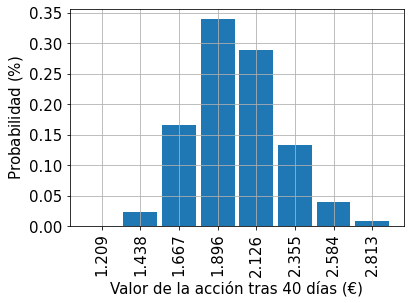
\includegraphics[width=\linewidth]{figures/notebooks/figure01.png}
    \caption{Representación gráfica de la variable \texttt{modelo\_incertidumbre}}
\end{figure}

\subsection{Algoritmo de estimación de la amplitud}
En la computación cuántica se consigue una mejora de la eficiencia respecto a los modelos clásicos con el algoritmo de Estimación de la amplitud.

Para un operador $\mathcal{A}$ que actúe en un registro de n+1 qubits tal que $\mathcal{A}|0\rangle_{n+1}=\sqrt{1-a}|\psi_0\rangle_n|0\rangle + \sqrt{a} |\psi_1\rangle|1\rangle$ donde $|\psi_0\rangle_n$ y $|\psi_0\rangle_n$ son estados normalizados y a pertenece a $[0,1]$. La estimación de amplitud estima el valor de a, que es la probabilidad de medir un $|1\rangle$. Esto lo hace con el operador $\mathcal{Q} = \mathcal{A}\mathcal{S}_0\mathcal{A}^\dagger\mathcal{S}_{\psi_0}$. Donde $S_0$ y $S_{\psi_0}$ son rotaciones, el algoritmo usa una estimación de fase (Quantum Phase Estimation) para conocer la fase de $\mathcal{Q}$ y la mapea a un estimador para $a$.  

Aunque es posible no usar la estimación de fase sabiendo que

\begin{align*}
\mathcal{Q}^k\mathcal{A}|0\rangle_n|0\rangle 
=& \cos\left(\left(2k+1\right)\theta_a\right)|\psi_0\rangle_n|0\rangle \\
+& \sin\left(\left(2k+1\right)\theta_a\right)|\psi_1\rangle_n|1\rangle
\end{align*}

\subsection{Implementación de la función de \textit{payoff}}
Pero el valor de la acción sólo nos interesa cuando es mayor que el \textit{strike price}, pues es cuando la función de pago retorna algún beneficio.

Como interesa considerar funciones lineales $f$ para cada qubit. Se usa un operador $\mathcal{A}$ tal que $a = \mathbb{E} [f(X)]$ (E es la esperanza matemática.

Se crea un operador que haga 

$$ |i\rangle_n|0\rangle \mapsto |i\rangle_n \left(\cos\left[f(i)\right]|0\rangle+\sin\left[f(i)\right]|1\rangle\right) $$

implementado mediante rotaciones Y controladas. 

A continuación queremos obtener $\mathbb{E}[f(X)]$, donde $f$ es una función lineal y $X$ es una variable aleatoria discretizada.

\begin{minted}{python}
precio_vencimiento = 1.896

# set the approximation scaling for the payoff function
c_approx = 0.25

# setup piecewise linear objective fcuntion
breakpoints = [bajo, precio_vencimiento]
slopes = [0, 1]
offsets = [0, 0]
f_min = 0
f_max = alto - precio_vencimiento
european_call_objective = LinearAmplitudeFunction(
    qubits,
    slopes,
    offsets,
    domain=(bajo, alto),
    image=(f_min, f_max),
    breakpoints=breakpoints,
    rescaling_factor=c_approx
)

num_qubits = european_call_objective.num_qubits
european_call = QuantumCircuit(num_qubits) 
european_call.append(modelo_incertidumbre, range(qubits))
european_call.append(european_call_objective, range(num_qubits))
\end{minted}

\begin{figure}[h]
    \centering
    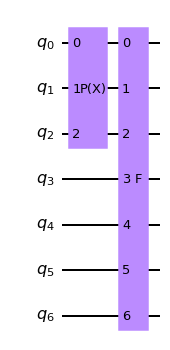
\includegraphics[height=5cm]{figures/notebooks/figura02.png}
    \caption{Visualización del circuito \texttt{european\_call}}
\end{figure}

\begin{figure}[h]
    \centering
    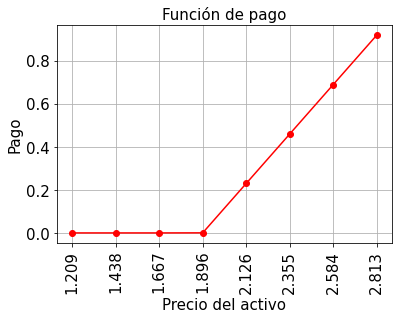
\includegraphics[width=\linewidth]{figures/notebooks/figura03.png}
    \caption{Visualización de la función de pago}
\end{figure}

\subsection{Evaluación del \textit{payoff} esperado}
Se compara el valor a partir del cual empieza a ser rentable la inversión del modelo con el del circuito que aplica la estimación de amplitud. En primer lugar usando el circuito implementado paso a paso para después compararlo con el circuito de la función del modulo finance de qiskit ``EuropeanCallExpectedValue'' para comprobar la precisión de ambos circuitos.

\begin{minted}{python}
epsilon = 0.01
alpha = 0.05

# construct amplitude estimation
ae = IterativeAmplitudeEstimation(
  epsilon=epsilon,alpha=alpha,
  state_preparation=european_call,
  objective_qubits=[3],
  post_processing=european_call_objective.post_processing
)

result = ae.run(quantum_instance=QasmSimulator()))

conf_int = np.array(result['confidence_interval'])
print('Exact value:        \t%.4f' % exact_value)
print('Estimated value:    \t%.4f' % (result['estimation']))
print('Confidence interval:\t[%.4f, %.4f]' % tuple(conf_int))
\end{minted}
\begin{resultado}
\begin{verbatim}
Exact value:        	0.1623
Estimated value:    	0.1698
Confidence interval:	[0.1637, 0.1760]
\end{verbatim}
\end{resultado}

\begin{minted}{python}
from qiskit.finance.applications import EuropeanCallExpectedValue

#Evalúa la opción call según el modelo proporcionado
european_call_objective = EuropeanCallExpectedValue(qubits,
    precio_vencimiento,
    rescaling_factor=c_approx,
    bounds=(bajo, alto))

european_cal1 = european_call_objective.compose(modelo_incertidumbre, front=True)

epsilon = 0.01
alpha = 0.05

ae = IterativeAmplitudeEstimation(
    epsilon=epsilon, alpha=alpha,
    state_preparation = european_cal1,
    objective_qubits = [3],
    post_processing = european_call_objective.post_processing)
result = ae.run(quantum_instance=QasmSimulator())

conf_int = np.array(result['confidence_interval'])
print('Exact value:        \t%.4f' % exact_value)
print('Estimated value:    \t%.4f' % (result['estimation']))
print('Confidence interval:\t[%.4f, %.4f]' % tuple(conf_int))
\end{minted}

\begin{resultado}
\begin{verbatim}
Exact value:        	0.1623
Estimated value:    	0.1704
Confidence interval:	[0.1620, 0.1789]
\end{verbatim}
\end{resultado}

Tras varias ejecuciones hemos observado que ambos circuitos parecen funcionar con la misma precisión y nos dan resultados parecidos.

\begin{minted}{python}
from qiskit.finance.applications import EuropeanCallDelta

european_call_delta = EuropeanCallDelta(qubits, precio_vencimiento, bounds=(bajo, alto))
state_preparation = QuantumCircuit(european_call_delta.num_qubits)
state_preparation.append(modelo_incertidumbre, range(modelo_incertidumbre.num_qubits))
state_preparation.append(european_call_delta, range(european_call_delta.num_qubits))
\end{minted}

\begin{figure}[h]
    \centering
    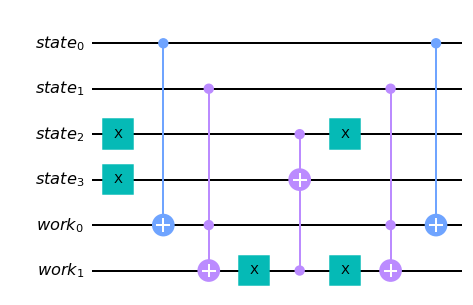
\includegraphics[width=\linewidth]{figures/notebooks/figura04.png}
    \caption{Visualización del circuito \texttt{european\_call\_delta}}
\end{figure}

\begin{figure}[h]
    \centering
    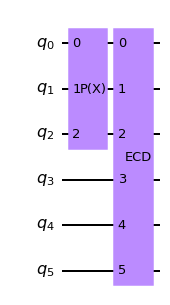
\includegraphics[height=5cm]{figures/notebooks/figura05.png}
    \caption{Visualización del circuito \texttt{state\_preparation}}
    \label{fig:my_label}
\end{figure}

\nocite{*}
\printbibliography

\end{document}
